\subsection{C.1 - Histerese }
Segue abaixo a implementação da simulção de histerese:
\begin{minted}{fortran}
            open(1, file="saidas/tarefa-3/saida-tarefa-C1-L60-DB1.dat")
            open(2, file="saidas/tarefa-3/saida-tarefa-C1-L60-DB2.dat")

            open(3, file="saidas/tarefa-3/saida-tarefa-C1-L80-DB1.dat")
            open(4, file="saidas/tarefa-3/saida-tarefa-C1-L80-DB2.dat")

            open(5, file="saidas/tarefa-3/saida-tarefa-C1-L100-DB1.dat")
            open(6, file="saidas/tarefa-3/saida-tarefa-C1-L100-DB2.dat")


            call tarefaC1(60, 0.001, 1)
            call tarefaC1(60, 0.0001,  2)

            call tarefaC1(80, 0.001, 3)
            call tarefaC1(80, 0.0001, 4)

            call tarefaC1(100,0.001, 5)
            call tarefaC1(100,0.0001, 6)

            do i = 1, 6
                close(i)
            end do
            end

            subroutine tarefaC1(L_real, dbeta, f_name)
                implicit integer(f-f)
            !           Tarefa B - Recozimento e quenching
                implicit real(j-j, m-m)
                parameter(L = 100)
                dimension exps(-4:4)
                byte lattice(1:L, 1:L)

                ! periodic boundary conditions
                dimension ipbc(0:L+1)

                do i = 1, L_real
                    ipbc(i) = i
                end do  

                ipbc(0) = L_real
                ipbc(L_real+1) = 1

                N = L_real * L_real

                mag = 0.0d0

                call srand(96312)
                ! b = 0
                call initialize_random_lattice(lattice,  L_real, L_real)

                call total_magnetization(lattice, mag, L_real)

                ! initial energy
                E = H_0(lattice, ipbc, L_real)

                beta = 0.0

                write(f_name, *) 0, beta,  mag, E/N

                imax = int(1.75 / dbeta) + 1 

                do i = 1, imax

                    call define_exponentials(exps, beta)

                    if(i < imax/ 2) then 
                        beta = beta + dbeta 
                    else
                        beta = beta - dbeta 
                    end if  

                    do k = 1 , N
                        call flip_spin(lattice,ipbc,exps,E,mag,L_real)
                    end do   

                    write(f_name, *) i, beta, mag, E/N

                end do
            end subroutine tarefaC1
\end{minted}


No gráfico (\ref{fig:c1_dbeta1}) temos o comportamento da energia média por spin na dinâmica do loop
térmico e o gráfico de histerese, isto é, a energia média em relação à $\beta$ para 
variações de $\Delta b = 0,001$. 

\begin{figure}
    \centering
    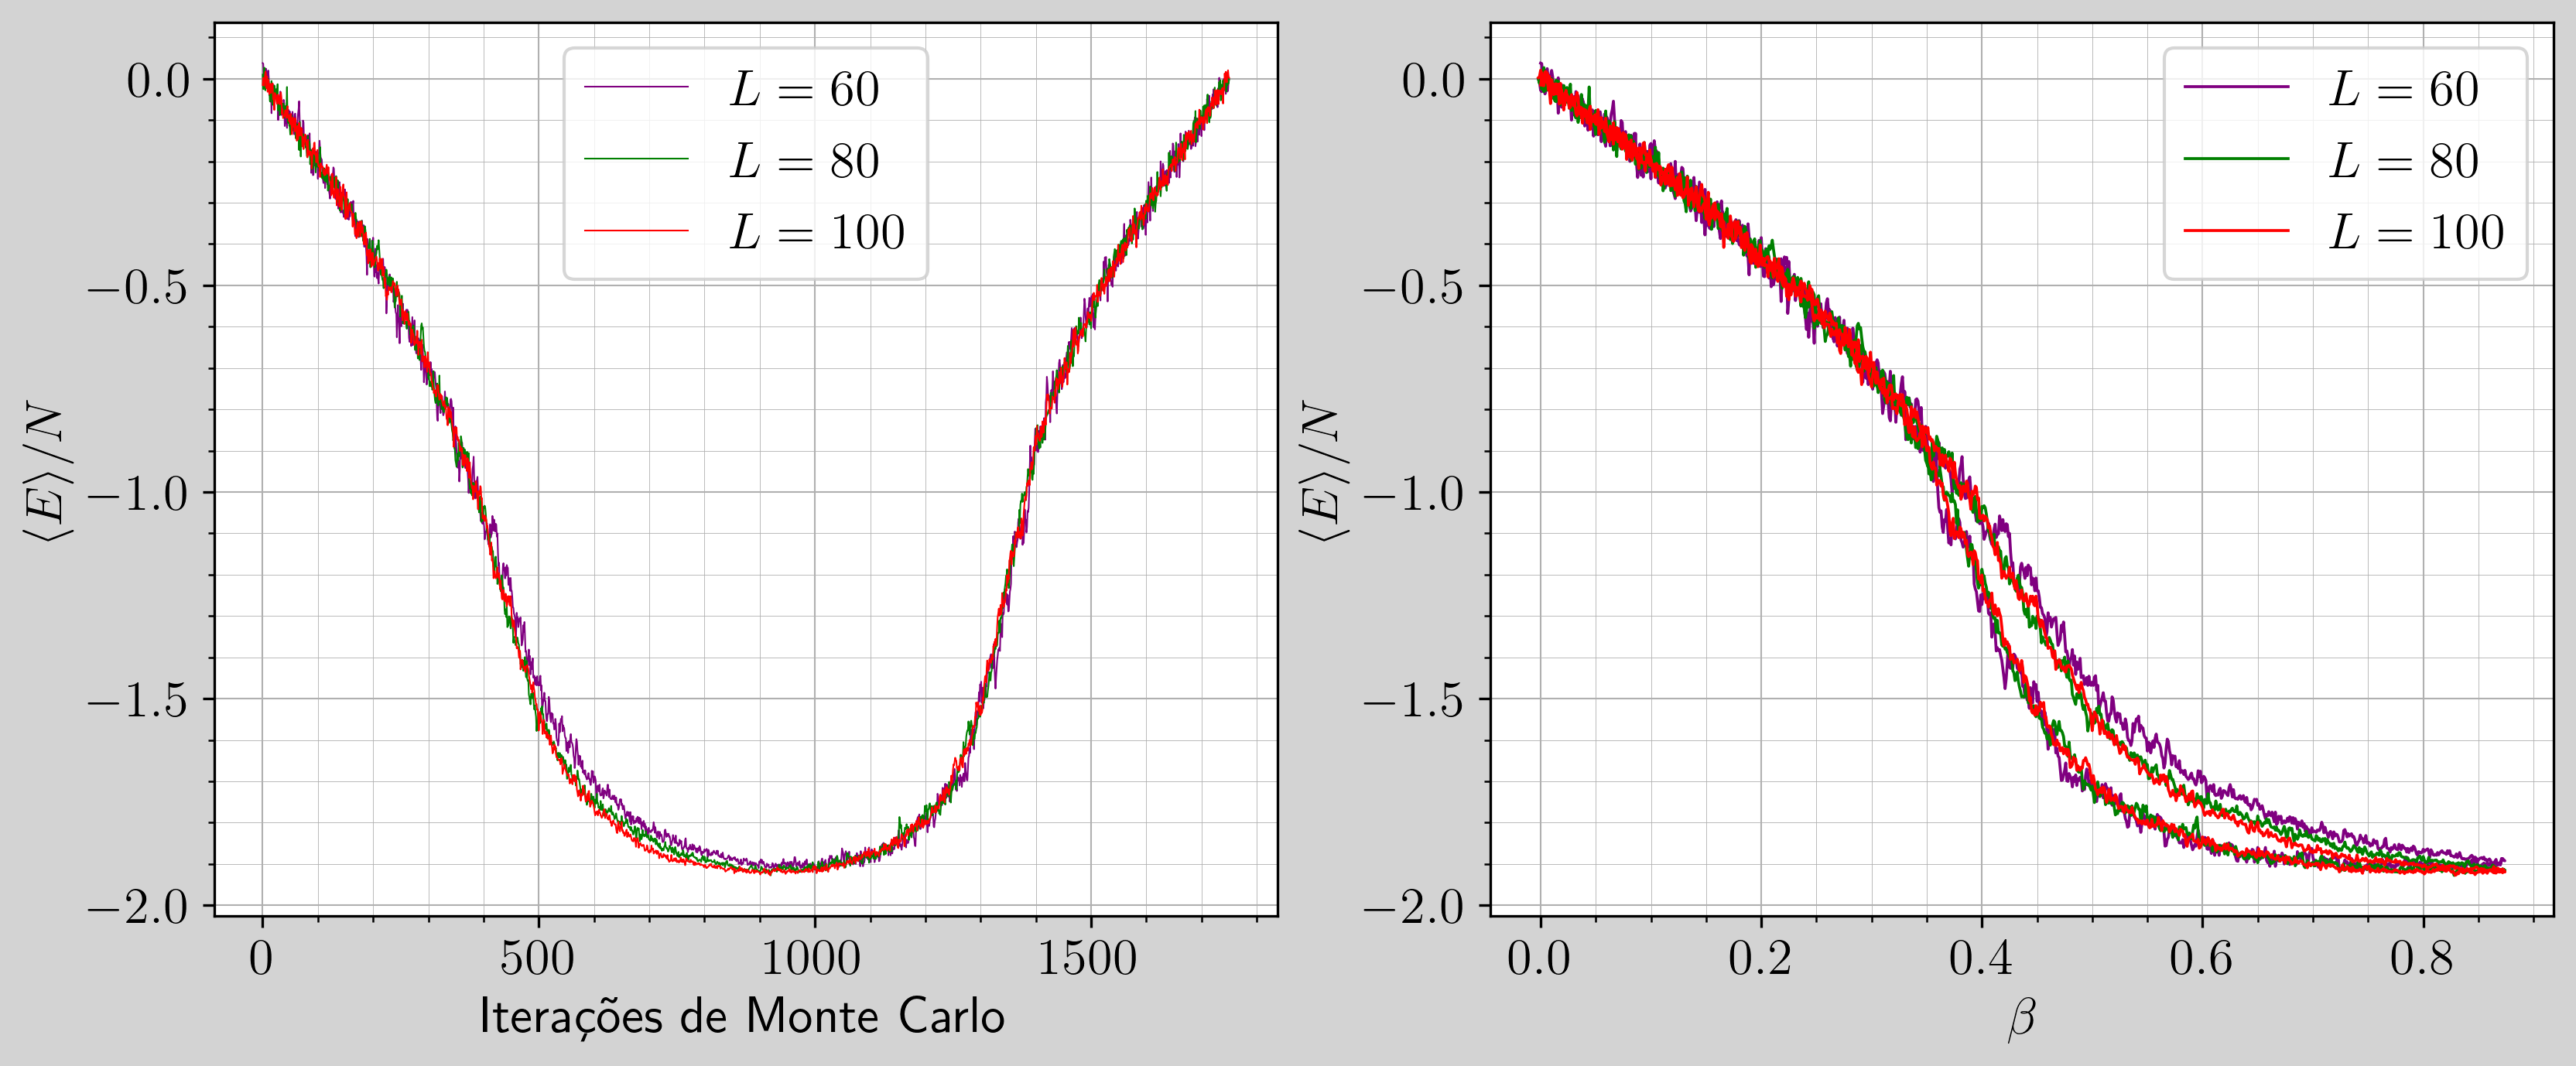
\includegraphics[width=0.8\linewidth]{graficos/tarefa-3/graf-tarefa-C1-delta1.png}
    \caption{À esquerda energia média por spin por iterações de Monte Carlo e à direita em relação à $\beta$.}
    \label{fig:c1_dbeta1}
\end{figure}


A figura (\ref{fig:c1_dbeta2}) equivale a dinâmica como a anterior, mas com uma variação 
$\Delta \beta = 0,0001$, que fornece um resultado com menos flutuações, sobretudo para as redes maiores.

\begin{figure}
    \centering
    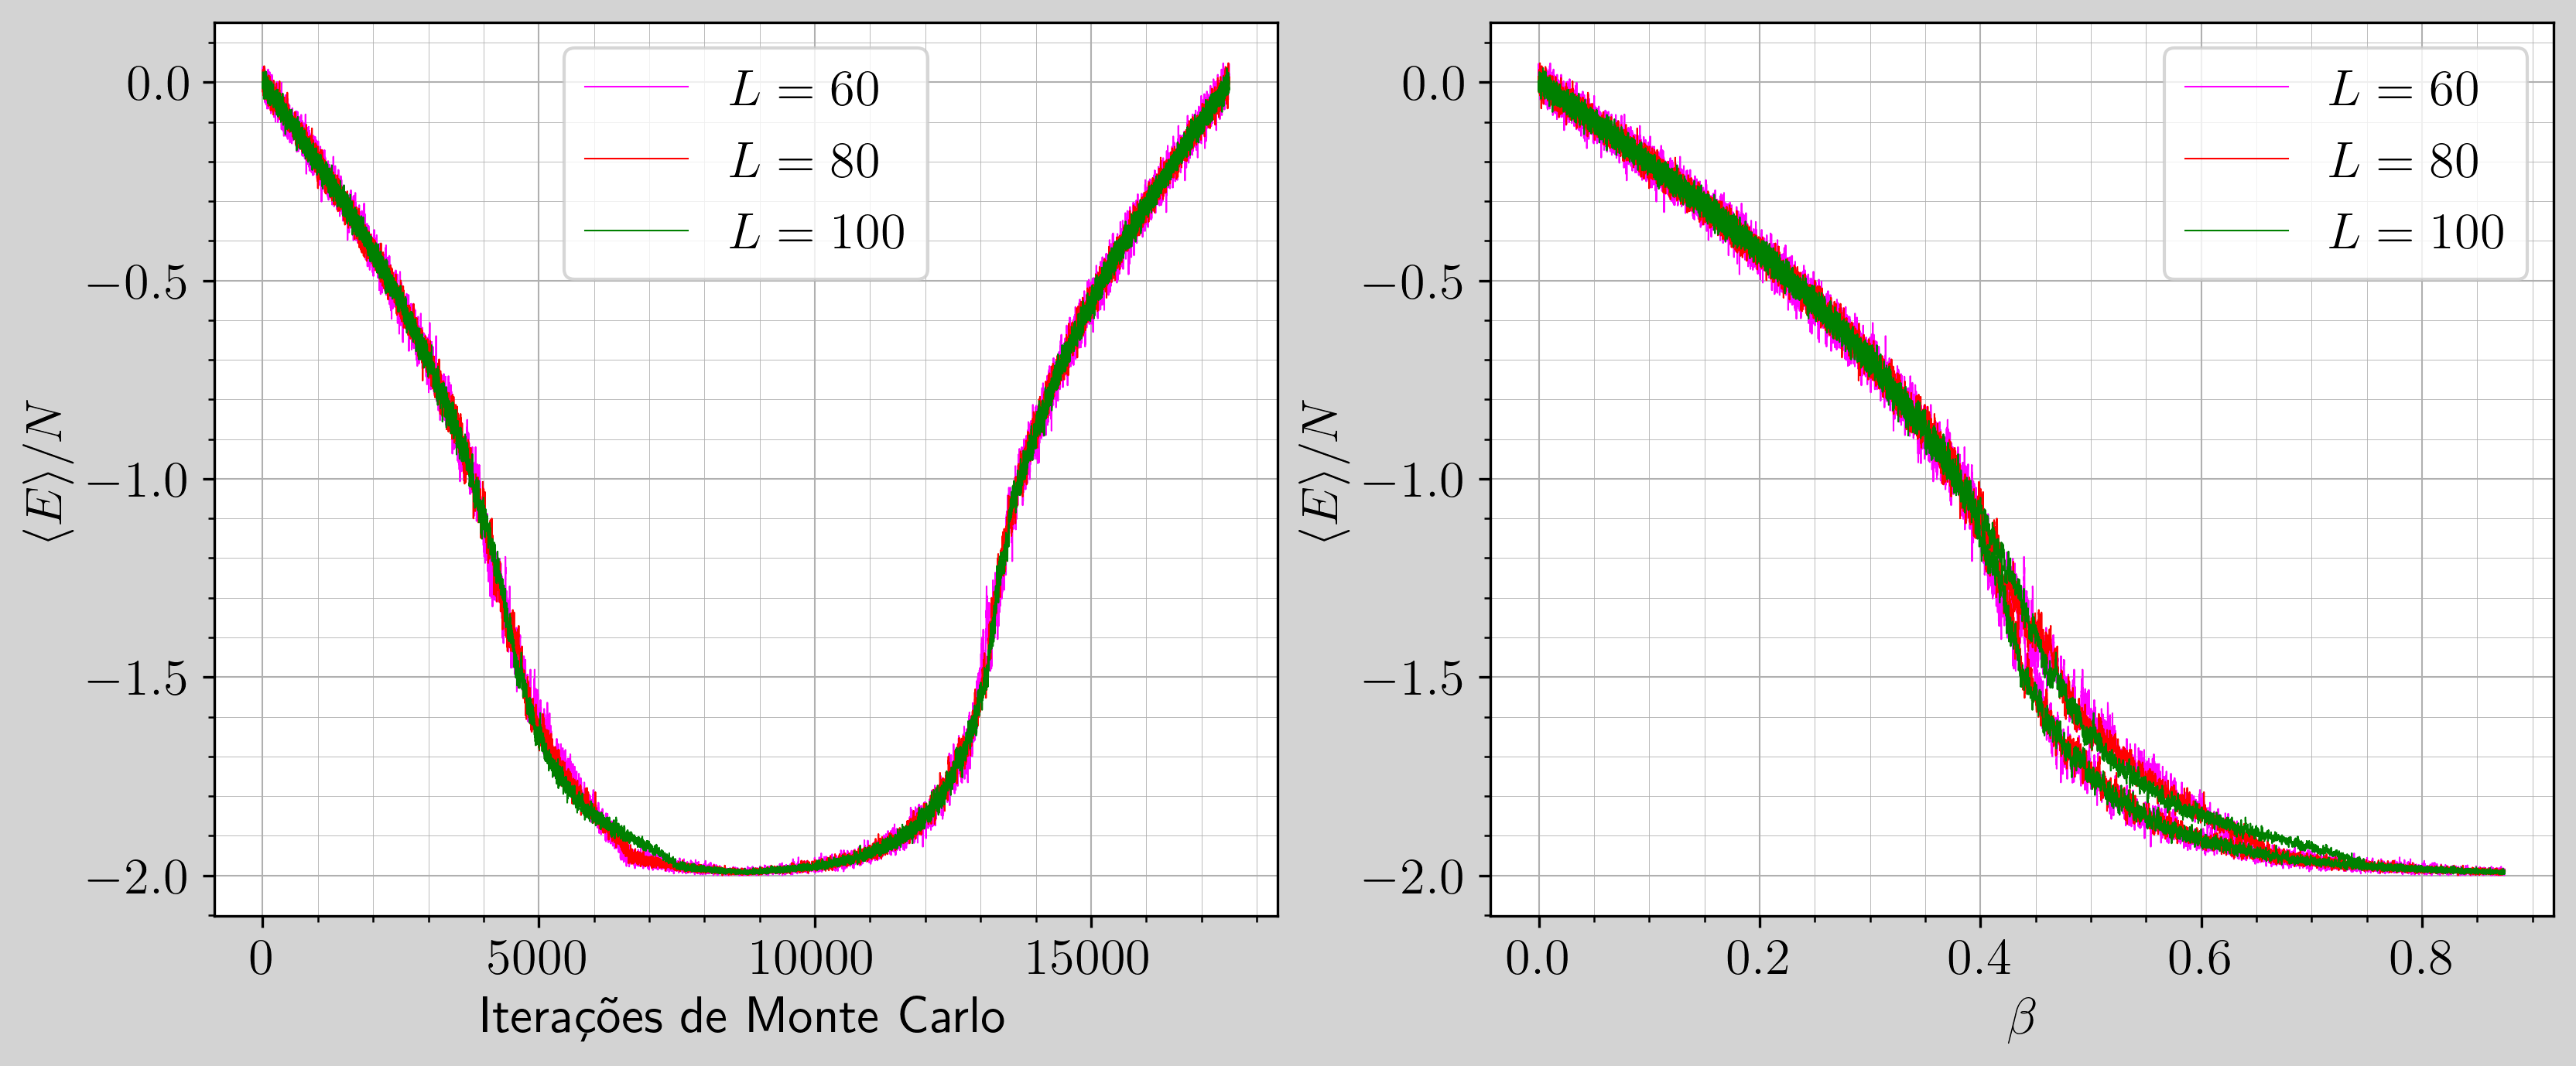
\includegraphics[width=0.8\linewidth]{graficos/tarefa-3/graf-tarefa-C1-delta2.png}
    \caption{À esquerda energia média por spin por iterações de Monte Carlo e à direita em relação à $\beta$.}
    \label{fig:c1_dbeta2}
\end{figure}

Podemos observar nos gráficos que a região de histerese correspondem à um intervalo de $\beta$ entre $0,4$ e 
$0,6$, mas apenas a partir dessas medidas não conseguimos ter uma boa precisão dessa medida.

\subsection{C.2 - Temperatura crítica }


\begin{marginfigure}
    \centering
    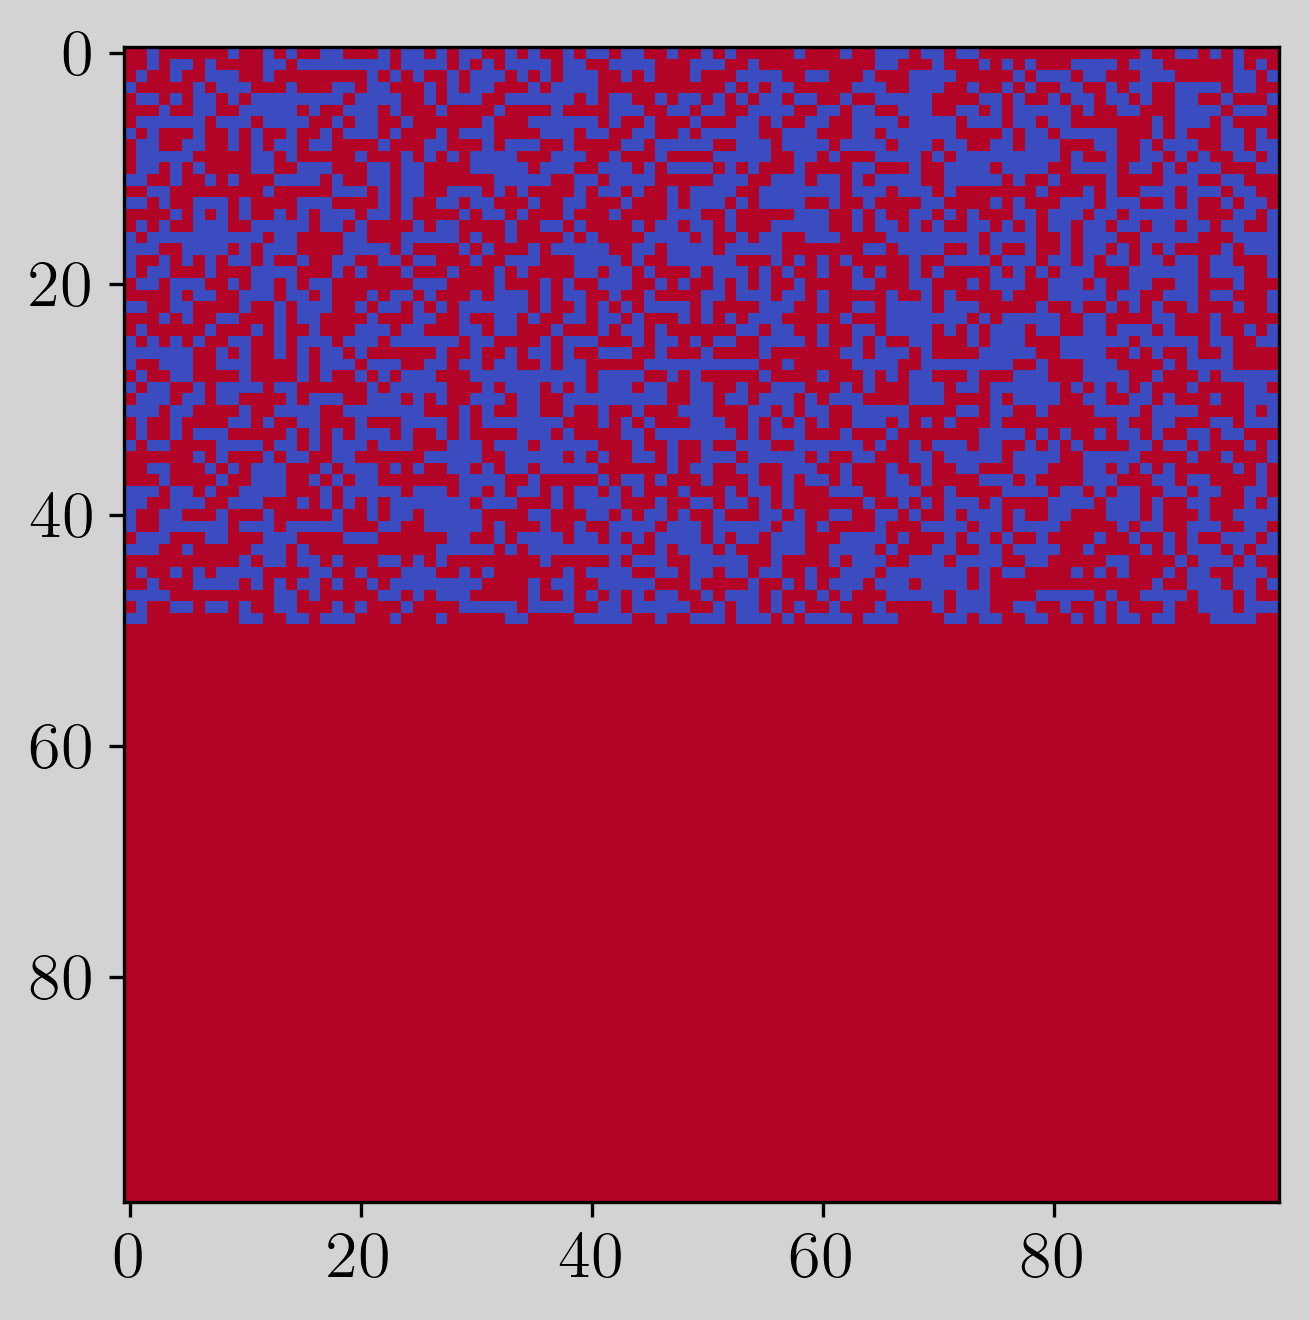
\includegraphics[width=\linewidth]{graficos/tarefa-3/graf-tarefa-C2-conf.png}
    \caption{Configuração inicial para dinâmica utilizada na medida de temperatura crítica.}
    \label{fig:c2_conf_inicial}
\end{marginfigure}


Modificação no código do item anterior: 

\begin{minted}{fortran}

        dimension betas(1:5)
        parameter(betas = (/0.41, 0.44, 0.47, 0.51, 0.55/))

        open(1, file="saidas/tarefa-3/saida-tarefa-C2-L60-b1.dat")
        open(2, file="saidas/tarefa-3/saida-tarefa-C2-L60-b2.dat")
        open(3, file="saidas/tarefa-3/saida-tarefa-C2-L60-b3.dat")
        open(4, file="saidas/tarefa-3/saida-tarefa-C2-L60-b4.dat")
        open(5, file="saidas/tarefa-3/saida-tarefa-C2-L60-b5.dat")

        do i = 1, 5
            call tarefaC2(60, betas(i), i)
            close(1)
        end do

        open(1, file="saidas/tarefa-3/saida-tarefa-C2-L80-b1.dat")
        open(2, file="saidas/tarefa-3/saida-tarefa-C2-L80-b2.dat")
        open(3, file="saidas/tarefa-3/saida-tarefa-C2-L80-b3.dat")
        open(4, file="saidas/tarefa-3/saida-tarefa-C2-L80-b4.dat")
        open(5, file="saidas/tarefa-3/saida-tarefa-C2-L80-b5.dat")

        do i = 1, 5
            call tarefaC2(80, betas(i), i)
            close(1)
        end do

        open(1, file="saidas/tarefa-3/saida-tarefa-C2-L100-b1.dat")
        open(2, file="saidas/tarefa-3/saida-tarefa-C2-L100-b2.dat")
        open(3, file="saidas/tarefa-3/saida-tarefa-C2-L100-b3.dat")
        open(4, file="saidas/tarefa-3/saida-tarefa-C2-L100-b4.dat")
        open(5, file="saidas/tarefa-3/saida-tarefa-C2-L100-b5.dat")

        do i = 1, 5
            call tarefaC2(100, betas(i), i)
            close(1)
        end do
        end
        subroutine tarefaC2(L_real, beta, fname)
!               Tarefa B - Recozimento e quenching
            implicit integer(f-f)
            implicit real(j-j, m-m)
            parameter(L = 100)
            dimension exps(-4:4)
            byte lattice(1:L, 1:L)
            ! periodic boundary conditions
            dimension ipbc(0:L+1)

            do i = 1, L_real
                ipbc(i) = i
            end do  

            ipbc(0) = L_real
            ipbc(L_real+1) = 1

            N = L_real * L_real

            mag = 0.0d0

            call srand(L_real * 392)

            ! half ordered / half random.
            call initialize_lattice(lattice, L_real, L_real)
            call initialize_random_lattice(lattice,  L_real/2, L_real)

            open(99, file = "saidas/tarefa-3/saida-tarefa-C2-conf.dat")
            call write_lattice(lattice, L_real, 99)
            close(99)

            call total_magnetization(lattice, mag, L_real)

            ! initial energy
            E = H_0(lattice, ipbc, L_real)
            dbeta = 0.01
            write(fname, *) 0, E/N
            do i = 1, 3000
                call define_exponentials(exps, beta)
                do k = 1 , N
                    call flip_spin(lattice,ipbc,exps,E,mag,L_real)
                end do   
                write(fname, *) i, E/N
            end do
        end subroutine tarefaC2
\end{minted}


\begin{marginfigure}
    \centering
    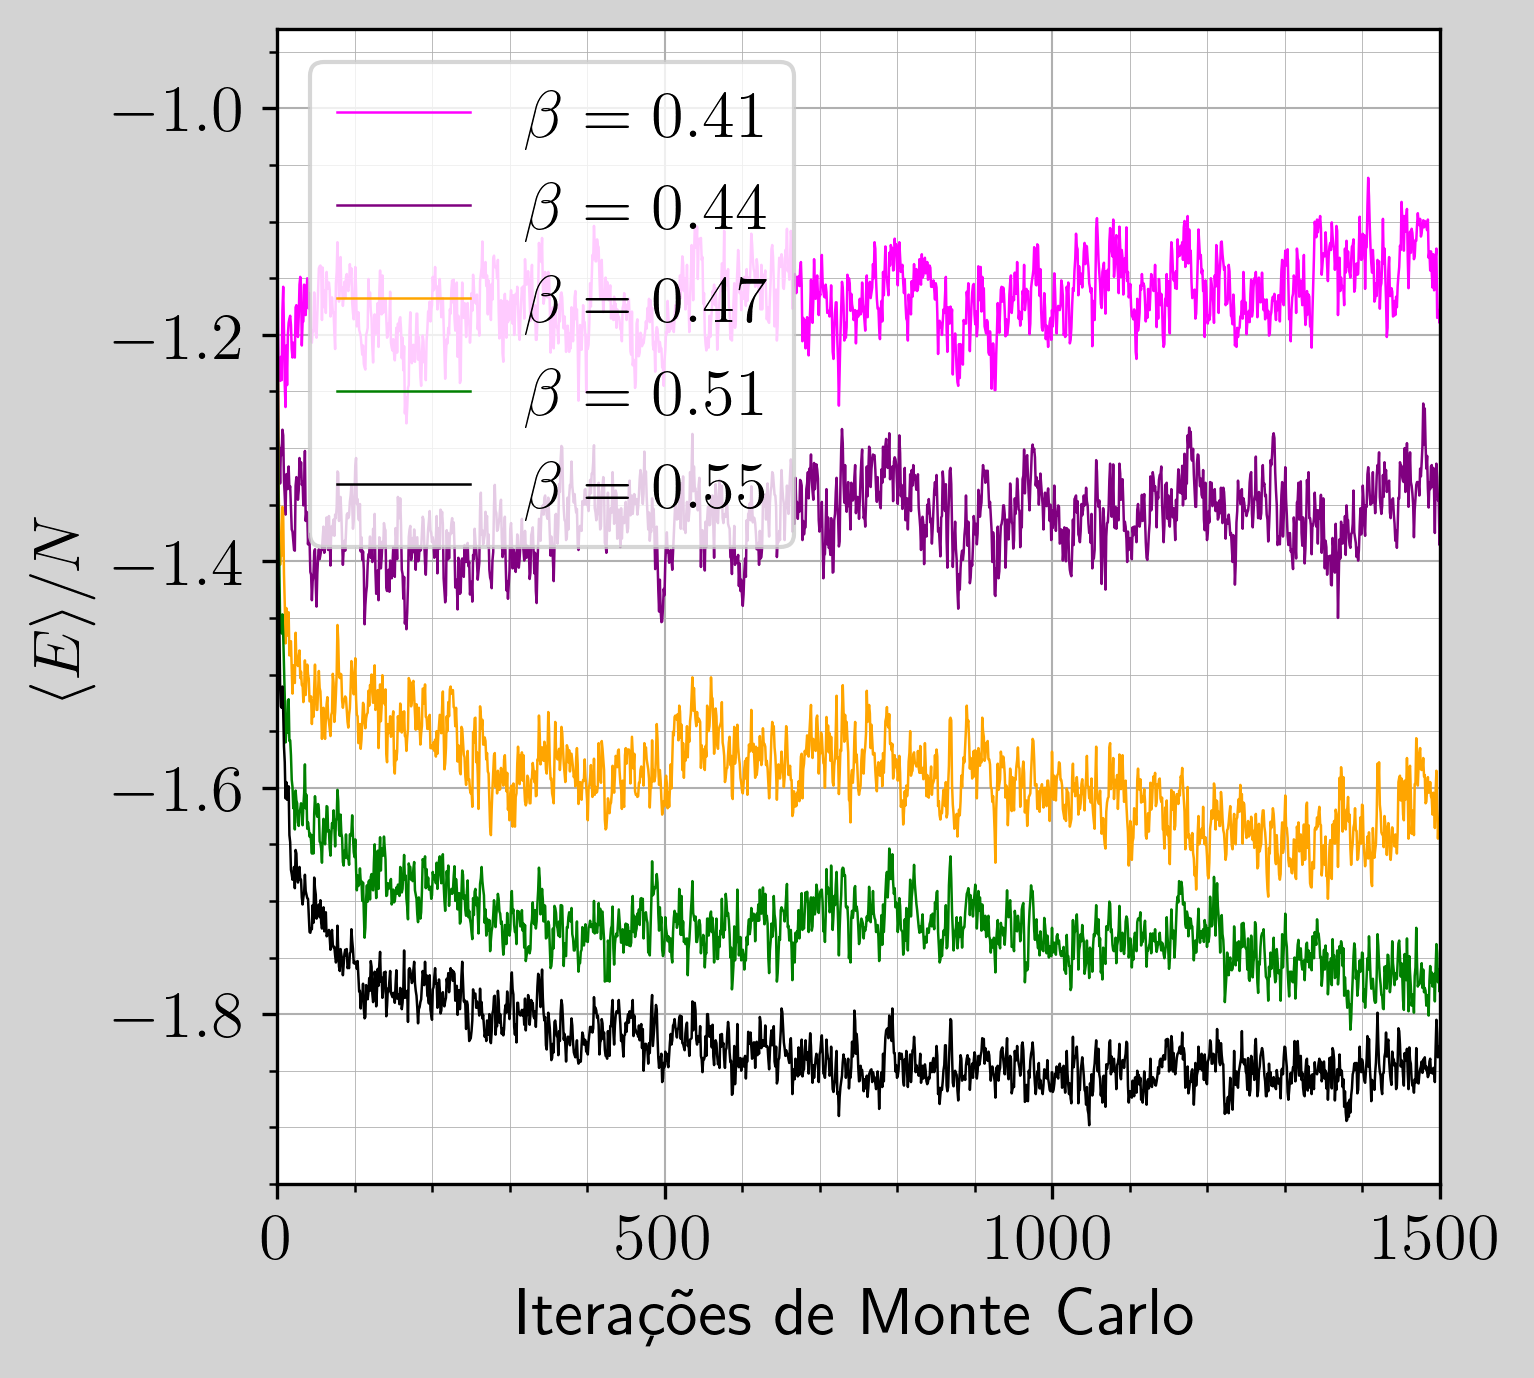
\includegraphics[width=\linewidth]{graficos/tarefa-3/graf-tarefa-C2-L80.png}
    \caption{Dinâmica para L=80.}
    \label{fig:c2_l80}
\end{marginfigure}

Partimos dos resultados do item anterior e tentamos obter a temperatura crítica do modelo. Para isso observamos
a variação de energia no intervalo $\beta$ discutido antes, isto é, $0,4 < \beta < 0.6$. 
A imagem (\ref{fig:c2_conf_inicial}) mostra a configuração inicial do sistema. Foram escolhidos alguns 
valores de $\beta$ para executar a dinâmica de Monte Carlo. 


\begin{marginfigure}
    \centering
    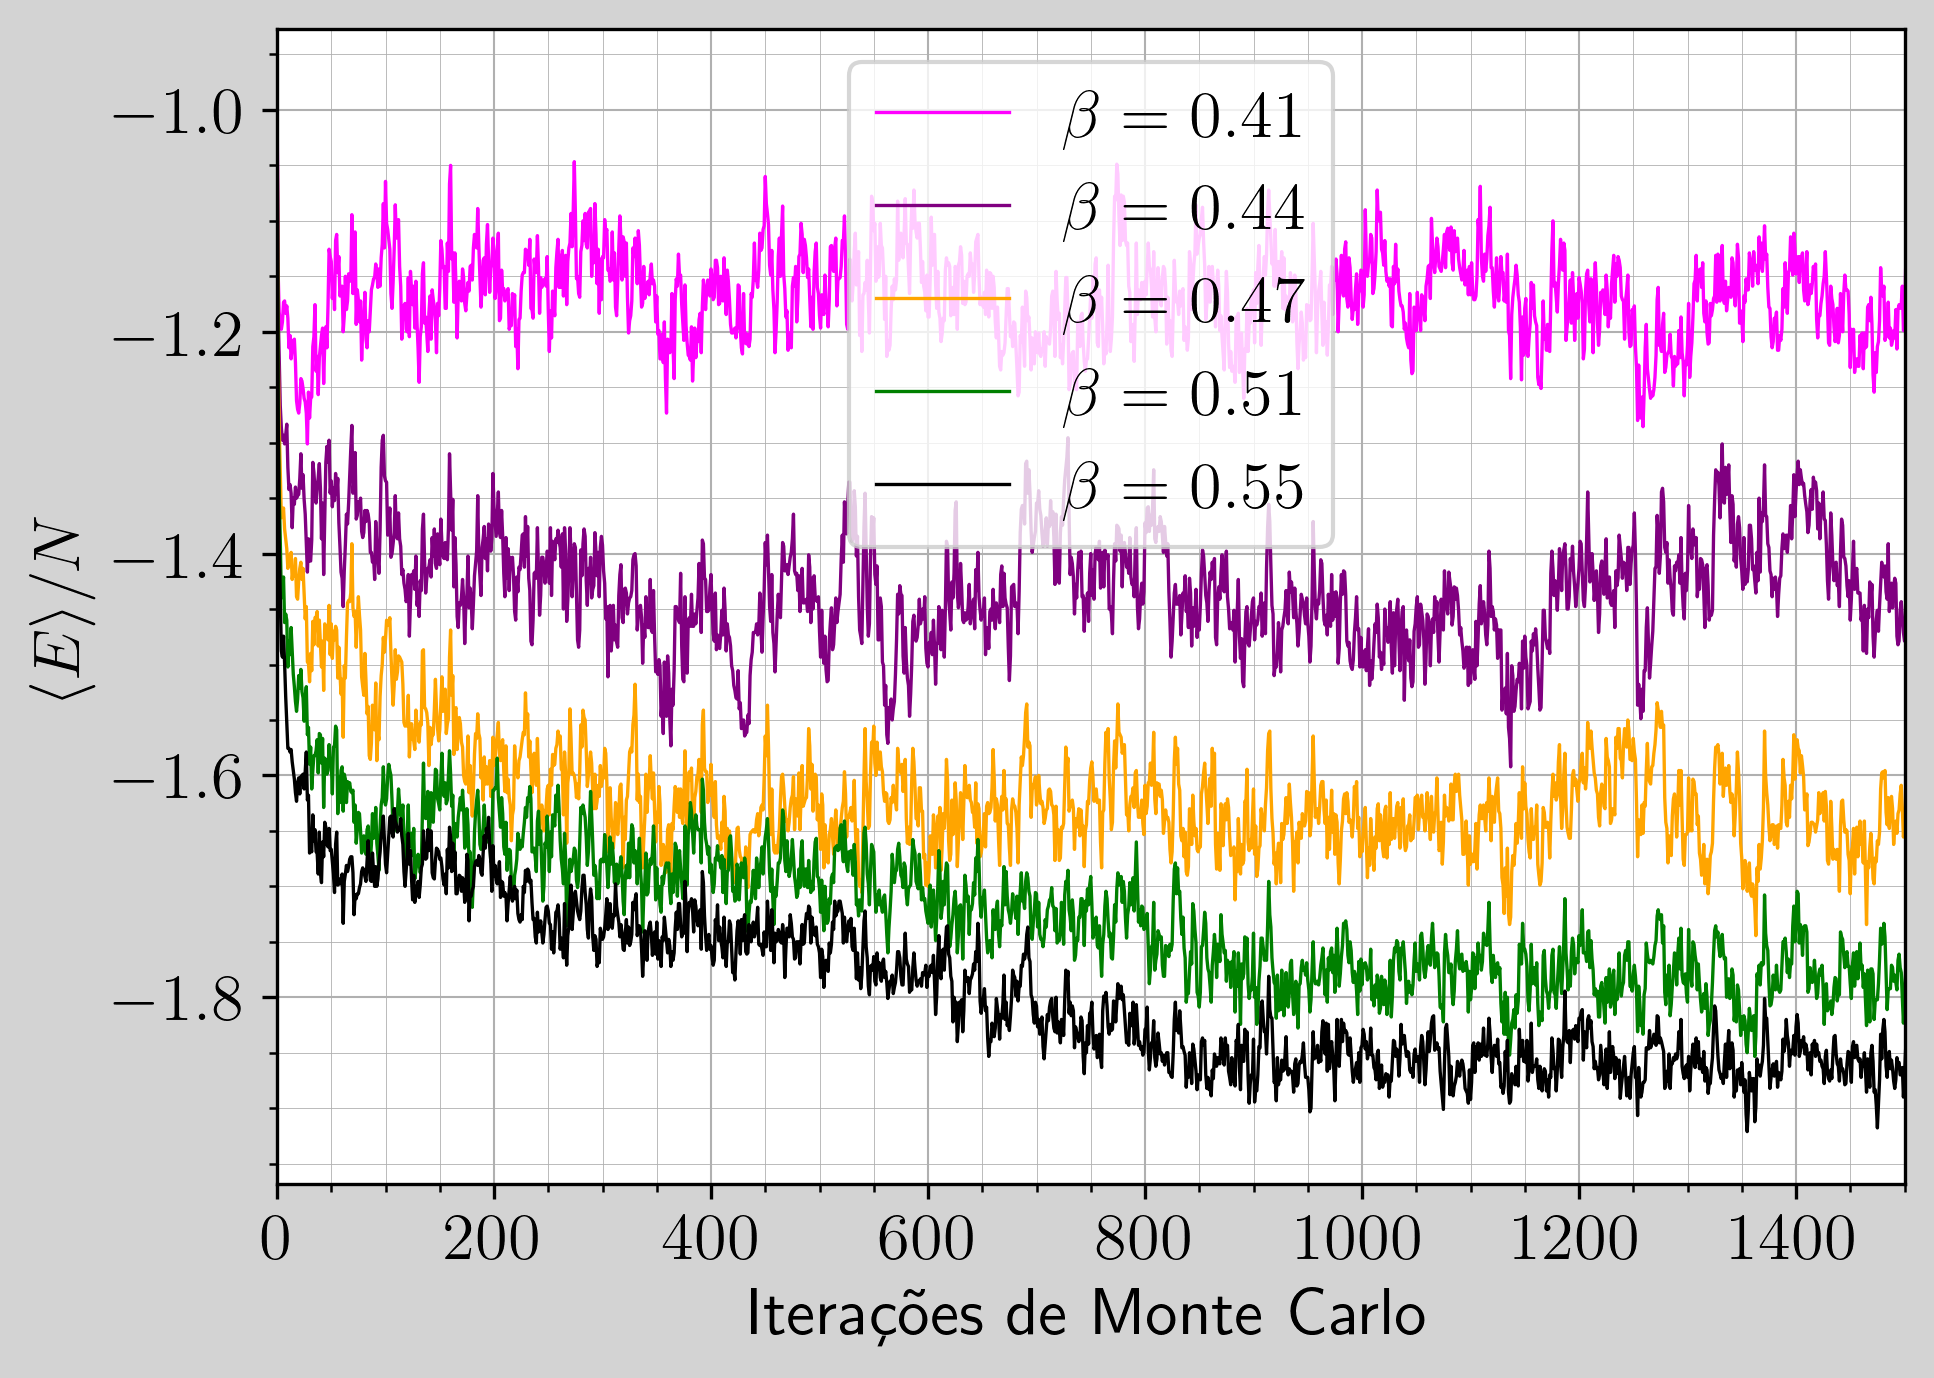
\includegraphics[width=\linewidth]{graficos/tarefa-3/graf-tarefa-C2-L60.png}
    \caption{Dinâmica para L=60.}
    \label{fig:c2_l60}
\end{marginfigure}



Nas figuras (\ref{fig:c2_l60}), (\ref{fig:c2_l80}) e (\ref{fig:c2_l100}) estão 
as evoluções, em um intervalo de passos de Monte Carlo reduzido, da energia média por spin. 

\clearpage
Nota-se que as energias médias por spin sempre partem do mesmo valor no intervalo da histerese e a 
que possui maior variação é a que corresponde à $\beta = 0.44$, esse é o $\beta$ relacionado à temperatura crítica $T_c = 1/\beta_c \approx 2,27$ .

\begin{figure}
    \centering
    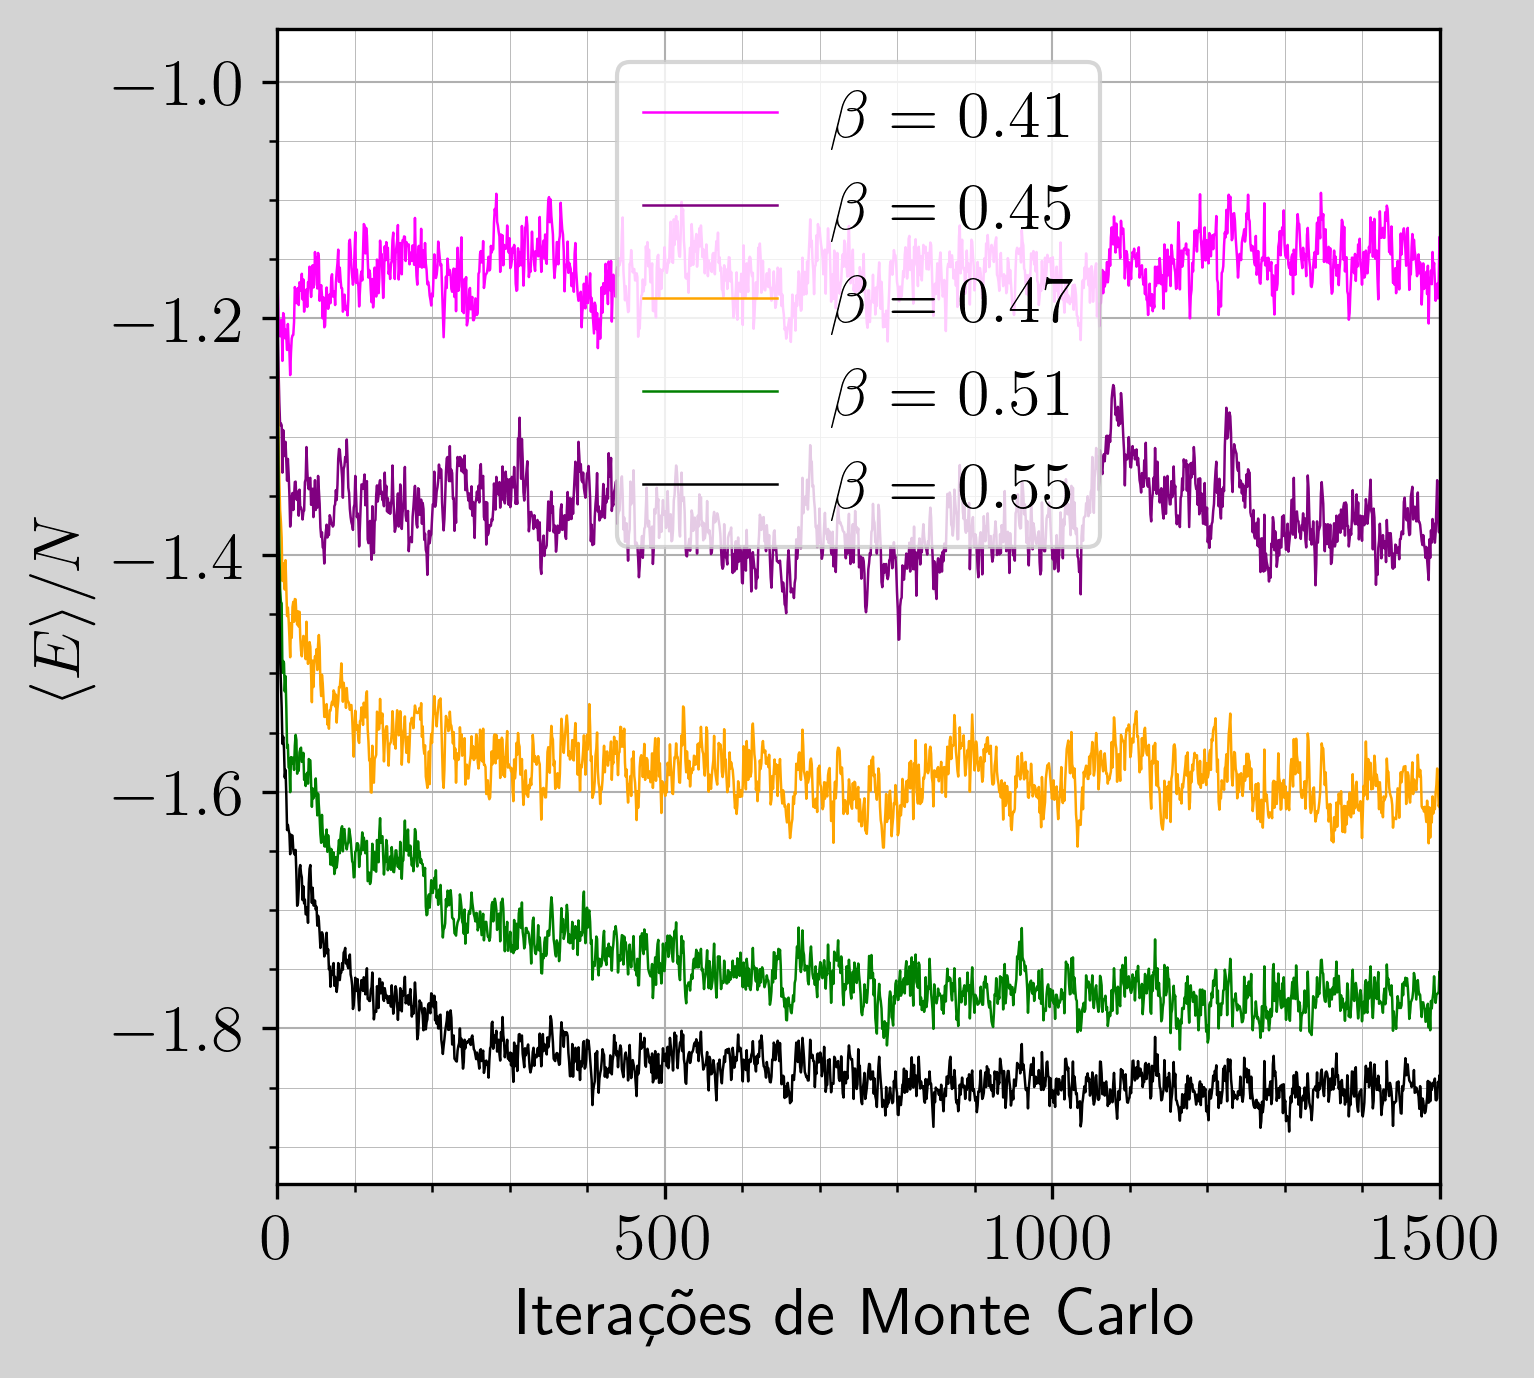
\includegraphics[width=0.5\linewidth]{graficos/tarefa-3/graf-tarefa-C2-L100.png}
    \caption{Dinâmica para L=100.}
    \label{fig:c2_l100}
\end{figure}

Além disso, pela (\ref{eq:calor_especifico}) podemos constatar que esse $\beta_c = 0,44$ também está associado à 
um valor específico crítico no modelo. 